\documentclass[border=10pt]{standalone}
\usepackage{tikz}
\usepackage{pgfplots}
\pgfplotsset{compat=1.17}

\begin{document}
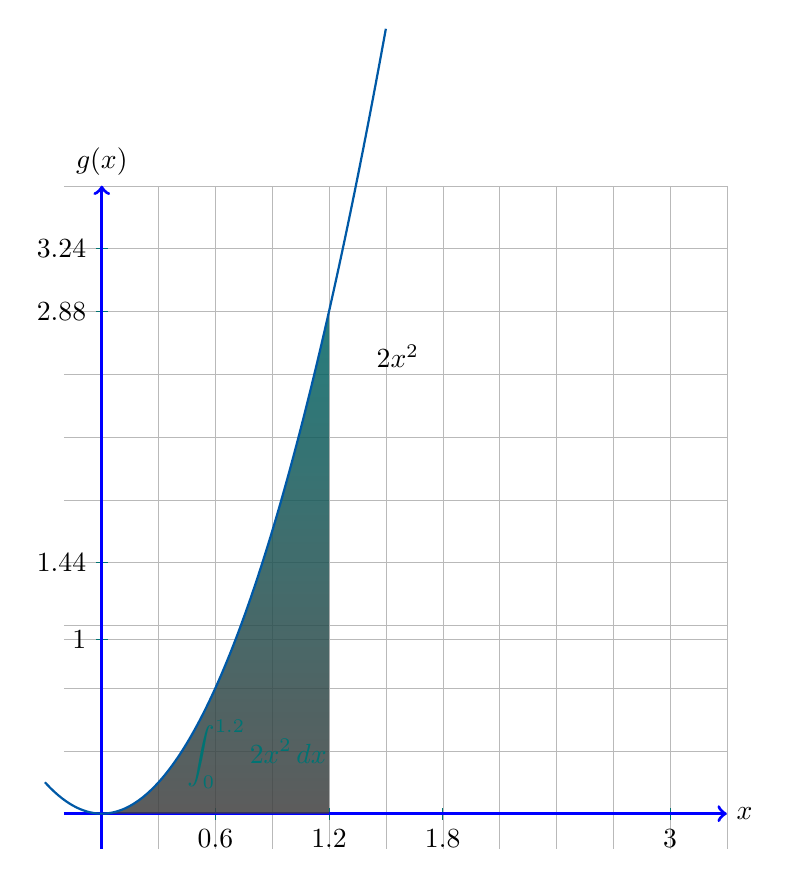
\begin{tikzpicture}
\begin{axis}[
    width=10cm,
    height=10cm,
    axis lines=middle,
    axis line style={blue, very thick, ->},
    xlabel={$x$},
    ylabel={$g(x)$},
    xlabel style={at={(axis description cs:1.0,-0.05)}, anchor=west},
    ylabel style={at={(axis description cs:-0.05,1.0)}, anchor=south},
    xmin=-0.2, xmax=3.3,
    ymin=-0.2, ymax=3.6,
    xtick={0.6, 1.2, 1.8, 3},
    ytick={1, 1.44, 2.88, 3.24},
    minor xtick={0,0.3,0.9,1.5,2.1,2.4,2.7,3.3},
    minor ytick={0,0.36,0.72,1.08,1.8,2.16,2.52,3.6},
    grid=both,
    grid style={line width=.1pt, draw=gray!55},
    minor grid style={line width=.1pt, draw=gray!55},
    tick style={teal!90!black},
    minor tick style={draw=none},
    every axis x label/.style={at={(ticklabel* cs:1.0)}, anchor=west},
    every axis y label/.style={at={(ticklabel* cs:1.0)}, anchor=south},
    samples=100,
    clip=false
]

% Shaded region under the curve
\addplot[
    domain=0:1.2,
    draw=none,
    shade,
    top color=teal!80!black,
    bottom color=black!75,
    opacity=0.85
] {2*x^2} \closedcycle;

% The curve 2x^2
\addplot[
    domain=-0.3:1.5,
    thick,
    teal!70!blue,
    smooth
] {2*x^2};

% Label for the curve
\node at (axis cs:1.4,2.5) [anchor=south west] {$2x^2$};

% Label for the shaded integral
\node at (axis cs:0.82,0.34) [teal!90!black] {$\displaystyle \int_0^{1.2} 2x^2\,dx$};

\end{axis}
\end{tikzpicture}
\end{document}
